\documentclass[11pt,a4paper]{article}

% ─── Packages ─────────────────────────────────────────────────────────────────
\usepackage[a4paper, margin=1in]{geometry}
\usepackage{graphicx}
\usepackage{booktabs}
\usepackage{caption}
\usepackage{float}
\usepackage{amsmath}
\usepackage{amsfonts}
\usepackage{amssymb}
\usepackage{hyperref}
\usepackage{xcolor}
\usepackage{array}
\usepackage{multirow}
\usepackage{tabularx}
\usepackage{longtable}
\usepackage{microtype}

\hypersetup{
    colorlinks=true,
    linkcolor=blue!70!black,
    citecolor=blue!70!black,
    urlcolor=blue!80!black
}

\title{\textbf{DLOps Assignment 5}\\[6pt]
       \large ViT-S LoRA Fine-Tuning on CIFAR-100 \&\\
       Adversarial Attacks with IBM ART on CIFAR-10}
\author{Vidhan Savaliya \\ \texttt{M25CSA031} \\ IIT Jodhpur}
\date{April 2026}

% ─── Document ─────────────────────────────────────────────────────────────────
\begin{document}

\maketitle
\tableofcontents
\newpage

% ─── Abstract ─────────────────────────────────────────────────────────────────
\section*{Abstract}
This report documents all experiments and results for Assignment 5 of the DLOps course. The assignment is divided into two parts:

\textbf{Q1} — Fine-tuning a pre-trained ViT-Small model on CIFAR-100 using Low-Rank Adaptation (LoRA) via PEFT. We evaluate 9 LoRA configurations (Ranks $\in \{2,4,8\}$, Alpha $\in \{2,4,8\}$, Dropout $= 0.1$) and use Optuna for best-hyperparameter search.

\textbf{Q2} — Adversarial robustness experiments on CIFAR-10 using a ResNet-18 trained from scratch and IBM Adversarial Robustness Toolbox (ART). Includes FGSM attacks from scratch and via ART, and binary adversarial detectors built on ResNet-34 using PGD and BIM attacks.

\bigskip
\noindent\textbf{Links:}
\begin{itemize}
  \item \textbf{WandB Q1:} \url{https://wandb.ai/vidhan-savaliya-indian-institute-of-technology-jodhpur/dlops-ass5-q1/overview}
  \item \textbf{WandB Q2:} \url{https://wandb.ai/vidhan-savaliya-indian-institute-of-technology-jodhpur/dlops-ass5-q2?nw=nwuservidhansavaliya}
  \item \textbf{HuggingFace Q1 Best LoRA:} \url{https://huggingface.co/Vidhansavaliya123/dlops-ass5-q1-vit-lora-best}
  \item \textbf{HuggingFace Q2 ResNet-18:} \url{https://huggingface.co/Vidhansavaliya123/dlops-ass5-q2-resnet18-cifar10}
\end{itemize}

\newpage

% ═══════════════════════════════════════════════════════════
\section{Question 1: ViT-S LoRA Fine-Tuning on CIFAR-100}
% ═══════════════════════════════════════════════════════════

\subsection{Setup and Methodology}

\paragraph{Model.} We use \texttt{vit\_small\_patch16\_224} pre-trained on ImageNet-21k from the \texttt{timm} library (total parameters: $\sim$21.7M). The classification head is replaced with a linear layer mapping to 100 classes.

\paragraph{LoRA Application.} We apply LoRA (via \texttt{peft}) to the combined QKV projection weight of every attention block. LoRA decomposes the weight update as $\Delta W = \frac{\alpha}{r} \cdot BA$, where $B \in \mathbb{R}^{d \times r}$, $A \in \mathbb{R}^{r \times d}$, $r$ is the rank, and $\alpha$ is the scaling factor. We experiment with:
\begin{itemize}
  \item \textbf{Ranks:} $r \in \{2, 4, 8\}$
  \item \textbf{Alpha:} $\alpha \in \{2, 4, 8\}$
  \item \textbf{Dropout:} $0.1$ (fixed)
\end{itemize}
This yields 9 LoRA configurations plus a baseline (frozen backbone, only classification head trained).

\paragraph{Training Details.}
\begin{itemize}
  \item Dataset: CIFAR-100 (45\,000 train / 5\,000 val / 10\,000 test), resized to $224\times224$ with ImageNet normalization.
  \item Optimizer: AdamW with cosine annealing LR schedule.
  \item Epochs: 10 per configuration.
  \item Mixed-precision (AMP) training on GPU.
\end{itemize}

\paragraph{Optuna.} We ran Optuna hyperparameter search over $\{$rank, alpha$\}$ to confirm the best configuration.

% ─────────────────────────────────────────────────────────────
\subsection{Per-Experiment Train/Validation Tables}

Below are the per-epoch results for all 10 experiments. The validation accuracy reported in each table is the \emph{best} checkpoint saved that epoch.

% ── Baseline ──────────────────────────────────────────────────
\subsubsection*{Experiment 0 — Baseline (No LoRA)}
\begin{center}
\small
LoRA Layers: \textbf{Without} \quad Trainable Params: \textbf{38,500} / 21,704,164
\end{center}

\begin{table}[H]
\centering
\begin{tabular}{@{}ccccc@{}}
\toprule
\textbf{Epoch} & \textbf{Train Loss} & \textbf{Val Loss} & \textbf{Train Acc (\%)} & \textbf{Val Acc (\%)} \\
\midrule
1  & 2.0691 & 1.6767 & 62.44 & 73.12 \\
2  & 1.7960 & 1.6248 & 70.40 & 75.04 \\
3  & 1.7619 & 1.6082 & 71.45 & 75.84 \\
4  & 1.7292 & 1.6117 & 72.28 & 75.72 \\
5  & 1.6960 & 1.5989 & 73.31 & 76.10 \\
6  & 1.6681 & 1.5870 & 74.43 & 76.56 \\
7  & 1.6513 & 1.5616 & 74.94 & 77.52 \\
8  & 1.6266 & 1.5511 & 75.94 & 77.96 \\
9  & 1.6066 & 1.5448 & 76.71 & 78.08 \\
10 & 1.5914 & 1.5405 & 77.11 & \textbf{78.12} \\
\bottomrule
\end{tabular}
\caption{Baseline — classification head only.}
\end{table}

% ── Exp 1 ─────────────────────────────────────────────────────
\subsubsection*{Experiment 1 — LoRA: Rank=2, Alpha=2, Dropout=0.1}
\begin{center}
\small Trainable Params: \textbf{75,364} / 21,779,528
\end{center}

\begin{table}[H]
\centering
\begin{tabular}{@{}ccccc@{}}
\toprule
\textbf{Epoch} & \textbf{Train Loss} & \textbf{Val Loss} & \textbf{Train Acc (\%)} & \textbf{Val Acc (\%)} \\
\midrule
1  & 1.5121 & 1.1957 & 78.53 & 87.72 \\
2  & 1.2022 & 1.1567 & 87.00 & 88.88 \\
3  & 1.1536 & 1.1407 & 88.60 & 89.36 \\
4  & 1.1222 & 1.1324 & 89.63 & 89.10 \\
5  & 1.0966 & 1.1232 & 90.58 & 89.58 \\
6  & 1.0767 & 1.1231 & 91.19 & 89.86 \\
7  & 1.0596 & 1.1179 & 91.90 & 89.62 \\
8  & 1.0459 & 1.1108 & 92.35 & 90.10 \\
9  & 1.0345 & 1.1092 & 92.88 & 90.20 \\
10 & 1.0292 & 1.1076 & 92.93 & \textbf{90.24} \\
\bottomrule
\end{tabular}
\caption{LoRA Exp 1: $r=2, \alpha=2$, dropout$=0.1$.}
\end{table}

% ── Exp 2 ─────────────────────────────────────────────────────
\subsubsection*{Experiment 2 — LoRA: Rank=2, Alpha=4, Dropout=0.1}
\begin{center}
\small Trainable Params: \textbf{75,364} / 21,779,528
\end{center}

\begin{table}[H]
\centering
\begin{tabular}{@{}ccccc@{}}
\toprule
\textbf{Epoch} & \textbf{Train Loss} & \textbf{Val Loss} & \textbf{Train Acc (\%)} & \textbf{Val Acc (\%)} \\
\midrule
1  & 1.5030 & 1.1884 & 78.58 & 87.30 \\
2  & 1.2009 & 1.1451 & 86.92 & 88.92 \\
3  & 1.1566 & 1.1408 & 88.40 & 89.18 \\
4  & 1.1198 & 1.1258 & 89.60 & 89.56 \\
5  & 1.0971 & 1.1339 & 90.58 & 89.24 \\
6  & 1.0751 & 1.1145 & 91.32 & 89.90 \\
7  & 1.0555 & 1.1121 & 91.90 & 89.88 \\
8  & 1.0398 & 1.1061 & 92.58 & 90.40 \\
9  & 1.0254 & 1.1050 & 93.01 & 90.22 \\
10 & 1.0235 & 1.1027 & 93.23 & \textbf{90.28} \\
\bottomrule
\end{tabular}
\caption{LoRA Exp 2: $r=2, \alpha=4$, dropout$=0.1$. Best val acc = 90.40\% at epoch 8.}
\end{table}

% ── Exp 3 ─────────────────────────────────────────────────────
\subsubsection*{Experiment 3 — LoRA: Rank=2, Alpha=8, Dropout=0.1}
\begin{center}
\small Trainable Params: \textbf{75,364} / 21,779,528
\end{center}

\begin{table}[H]
\centering
\begin{tabular}{@{}ccccc@{}}
\toprule
\textbf{Epoch} & \textbf{Train Loss} & \textbf{Val Loss} & \textbf{Train Acc (\%)} & \textbf{Val Acc (\%)} \\
\midrule
1  & 1.4946 & 1.1974 & 78.97 & 87.08 \\
2  & 1.2036 & 1.1660 & 86.72 & 88.84 \\
3  & 1.1586 & 1.1498 & 88.27 & 88.90 \\
4  & 1.1283 & 1.1317 & 89.33 & 89.14 \\
5  & 1.1029 & 1.1240 & 90.15 & 89.38 \\
6  & 1.0753 & 1.1167 & 91.16 & 90.00 \\
7  & 1.0562 & 1.1090 & 91.78 & 90.04 \\
8  & 1.0375 & 1.1066 & 92.58 & 90.22 \\
9  & 1.0268 & 1.0985 & 92.94 & \textbf{90.50} \\
10 & 1.0188 & 1.1001 & 93.16 & 90.42 \\
\bottomrule
\end{tabular}
\caption{LoRA Exp 3: $r=2, \alpha=8$, dropout$=0.1$.}
\end{table}

% ── Exp 4 ─────────────────────────────────────────────────────
\subsubsection*{Experiment 4 — LoRA: Rank=4, Alpha=2, Dropout=0.1}
\begin{center}
\small Trainable Params: \textbf{112,228} / 21,816,392
\end{center}

\begin{table}[H]
\centering
\begin{tabular}{@{}ccccc@{}}
\toprule
\textbf{Epoch} & \textbf{Train Loss} & \textbf{Val Loss} & \textbf{Train Acc (\%)} & \textbf{Val Acc (\%)} \\
\midrule
1  & 1.5007 & 1.1843 & 78.81 & 87.66 \\
2  & 1.1949 & 1.1450 & 87.15 & 89.12 \\
3  & 1.1410 & 1.1352 & 88.89 & 89.34 \\
4  & 1.1101 & 1.1204 & 89.95 & 90.26 \\
5  & 1.0823 & 1.1142 & 90.92 & 90.24 \\
6  & 1.0604 & 1.1022 & 91.73 & 90.70 \\
7  & 1.0415 & 1.1014 & 92.34 & 90.68 \\
8  & 1.0278 & 1.0979 & 92.90 & \textbf{90.78} \\
9  & 1.0153 & 1.0945 & 93.37 & 90.68 \\
10 & 1.0085 & 1.0935 & 93.64 & 90.78 \\
\bottomrule
\end{tabular}
\caption{LoRA Exp 4: $r=4, \alpha=2$, dropout$=0.1$.}
\end{table}

% ── Exp 5 — Best ──────────────────────────────────────────────
\subsubsection*{Experiment 5 — LoRA: Rank=4, Alpha=4, Dropout=0.1 \textnormal{(\textbf{Best / Optuna-selected})}}
\begin{center}
\small Trainable Params: \textbf{112,228} / 21,816,392
\end{center}

\begin{table}[H]
\centering
\begin{tabular}{@{}ccccc@{}}
\toprule
\textbf{Epoch} & \textbf{Train Loss} & \textbf{Val Loss} & \textbf{Train Acc (\%)} & \textbf{Val Acc (\%)} \\
\midrule
1  & 1.4837 & 1.1778 & 79.12 & 88.04 \\
2  & 1.1932 & 1.1515 & 87.06 & 88.64 \\
3  & 1.1375 & 1.1460 & 88.89 & 89.02 \\
4  & 1.1010 & 1.1199 & 90.19 & 89.62 \\
5  & 1.0755 & 1.1138 & 91.09 & 90.36 \\
6  & 1.0546 & 1.1048 & 91.84 & 90.14 \\
7  & 1.0298 & 1.0995 & 92.83 & 90.18 \\
8  & 1.0160 & 1.0966 & 93.28 & 90.50 \\
9  & 1.0049 & 1.0914 & 93.70 & \textbf{90.88} \\
10 & 1.0085 & 1.0935 & 93.64 & 90.78 \\
\bottomrule
\end{tabular}
\caption{LoRA Exp 5 (\textbf{Best}): $r=4, \alpha=4$, dropout$=0.1$. Best validation accuracy = \textbf{90.88\%}.}
\end{table}

% ── Exp 6 ─────────────────────────────────────────────────────
\subsubsection*{Experiment 6 — LoRA: Rank=4, Alpha=8, Dropout=0.1}
\begin{center}
\small Trainable Params: \textbf{112,228} / 21,816,392
\end{center}

\begin{table}[H]
\centering
\begin{tabular}{@{}ccccc@{}}
\toprule
\textbf{Epoch} & \textbf{Train Loss} & \textbf{Val Loss} & \textbf{Train Acc (\%)} & \textbf{Val Acc (\%)} \\
\midrule
1  & 1.4764 & 1.1732 & 79.29 & 88.22 \\
2  & 1.1881 & 1.1387 & 87.37 & 88.92 \\
3  & 1.1394 & 1.1315 & 88.80 & 88.84 \\
4  & 1.1043 & 1.1166 & 90.00 & 89.74 \\
5  & 1.0756 & 1.1095 & 91.10 & 89.84 \\
6  & 1.0488 & 1.1045 & 91.99 & 90.32 \\
7  & 1.0262 & 1.0953 & 92.74 & 90.64 \\
8  & 1.0091 & 1.0956 & 93.53 & 90.46 \\
9  & 0.9968 & 1.0878 & 93.98 & \textbf{90.80} \\
10 & 0.9879 & 1.0853 & 94.23 & 90.80 \\
\bottomrule
\end{tabular}
\caption{LoRA Exp 6: $r=4, \alpha=8$, dropout$=0.1$.}
\end{table}

% ── Exp 7 ─────────────────────────────────────────────────────
\subsubsection*{Experiment 7 — LoRA: Rank=8, Alpha=2, Dropout=0.1}
\begin{center}
\small Trainable Params: \textbf{185,956} / 21,890,120
\end{center}

\begin{table}[H]
\centering
\begin{tabular}{@{}ccccc@{}}
\toprule
\textbf{Epoch} & \textbf{Train Loss} & \textbf{Val Loss} & \textbf{Train Acc (\%)} & \textbf{Val Acc (\%)} \\
\midrule
1  & 1.5017 & 1.1868 & 78.56 & 87.68 \\
2  & 1.1897 & 1.1410 & 87.26 & 89.00 \\
3  & 1.1336 & 1.1292 & 89.18 & 89.04 \\
4  & 1.1009 & 1.1133 & 90.28 & 90.00 \\
5  & 1.0714 & 1.1090 & 91.22 & 90.20 \\
6  & 1.0455 & 1.1049 & 92.22 & 90.26 \\
7  & 1.0284 & 1.1020 & 92.79 & 90.12 \\
8  & 1.0146 & 1.0990 & 93.32 & 90.42 \\
9  & 1.0042 & 1.0944 & 93.80 & \textbf{90.54} \\
10 & 0.9962 & 1.0933 & 94.09 & 90.54 \\
\bottomrule
\end{tabular}
\caption{LoRA Exp 7: $r=8, \alpha=2$, dropout$=0.1$.}
\end{table}

% ── Exp 8 ─────────────────────────────────────────────────────
\subsubsection*{Experiment 8 — LoRA: Rank=8, Alpha=4, Dropout=0.1}
\begin{center}
\small Trainable Params: \textbf{185,956} / 21,890,120
\end{center}

\begin{table}[H]
\centering
\begin{tabular}{@{}ccccc@{}}
\toprule
\textbf{Epoch} & \textbf{Train Loss} & \textbf{Val Loss} & \textbf{Train Acc (\%)} & \textbf{Val Acc (\%)} \\
\midrule
1  & 1.4779 & 1.1645 & 79.52 & 88.58 \\
2  & 1.1808 & 1.1404 & 87.40 & 88.90 \\
3  & 1.1252 & 1.1207 & 89.27 & 89.44 \\
4  & 1.0870 & 1.1121 & 90.62 & 89.78 \\
5  & 1.0588 & 1.1036 & 91.67 & 90.16 \\
6  & 1.0339 & 1.0975 & 92.46 & 90.36 \\
7  & 1.0104 & 1.0913 & 93.30 & 90.56 \\
8  & 0.9953 & 1.0853 & 93.98 & 90.46 \\
9  & 0.9829 & 1.0834 & 94.36 & \textbf{90.66} \\
10 & 0.9791 & 1.0821 & 94.58 & 90.62 \\
\bottomrule
\end{tabular}
\caption{LoRA Exp 8: $r=8, \alpha=4$, dropout$=0.1$.}
\end{table}

% ── Exp 9 ─────────────────────────────────────────────────────
\subsubsection*{Experiment 9 — LoRA: Rank=8, Alpha=8, Dropout=0.1}
\begin{center}
\small Trainable Params: \textbf{185,956} / 21,890,120
\end{center}

\begin{table}[H]
\centering
\begin{tabular}{@{}ccccc@{}}
\toprule
\textbf{Epoch} & \textbf{Train Loss} & \textbf{Val Loss} & \textbf{Train Acc (\%)} & \textbf{Val Acc (\%)} \\
\midrule
1  & 1.4741 & 1.1733 & 79.45 & 87.44 \\
2  & 1.1764 & 1.1390 & 87.72 & 88.92 \\
3  & 1.1236 & 1.1304 & 89.30 & 89.48 \\
4  & 1.0821 & 1.1156 & 90.75 & 89.92 \\
5  & 1.0517 & 1.1114 & 91.76 & 90.22 \\
6  & 1.0200 & 1.1038 & 92.86 & 90.28 \\
7  & 1.0008 & 1.0942 & 93.55 & 90.66 \\
8  & 0.9791 & 1.0891 & 94.42 & 90.50 \\
9  & 0.9667 & 1.0900 & 94.90 & \textbf{90.84} \\
10 & 0.9579 & 1.0861 & 95.23 & 90.84 \\
\bottomrule
\end{tabular}
\caption{LoRA Exp 9: $r=8, \alpha=8$, dropout$=0.1$.}
\end{table}

% ─────────────────────────────────────────────────────────────
\subsection{Overall Test Accuracy — Summary Table}

\begin{table}[H]
\centering
\begin{tabular}{@{}llccccc@{}}
\toprule
\textbf{Exp} & \textbf{LoRA Layers} & \textbf{Rank} & \textbf{Alpha} & \textbf{Dropout} & \textbf{Test Acc (\%)} & \textbf{Trainable Params} \\
\midrule
0 & Without & --- & --- & ---  & 78.12 & 38,500 \\
1 & With    & 2   & 2   & 0.1  & 90.24 & 75,364 \\
2 & With    & 2   & 4   & 0.1  & 90.40 & 75,364 \\
3 & With    & 2   & 8   & 0.1  & 90.50 & 75,364 \\
4 & With    & 4   & 2   & 0.1  & 90.78 & 112,228 \\
\textbf{5} & \textbf{With} & \textbf{4} & \textbf{4} & \textbf{0.1} & \textbf{90.88} & \textbf{112,228} \\
6 & With    & 4   & 8   & 0.1  & 90.80 & 112,228 \\
7 & With    & 8   & 2   & 0.1  & 90.54 & 185,956 \\
8 & With    & 8   & 4   & 0.1  & 90.66 & 185,956 \\
9 & With    & 8   & 8   & 0.1  & 90.84 & 185,956 \\
\bottomrule
\end{tabular}
\caption{Overall test accuracy for all configurations. \textbf{Bold} = Optuna-selected best.}
\end{table}

% ─────────────────────────────────────────────────────────────
\subsection{Optuna Hyperparameter Search}

Optuna was used to search over $r \in \{2,4,8\}$ and $\alpha \in \{2,4,8\}$ (with dropout fixed at 0.1). The best trial confirmed $r=4, \alpha=4$, yielding a peak validation accuracy of \textbf{90.88\%}. This configuration provides the optimal trade-off between adaptation capacity and parameter efficiency:
\begin{itemize}
  \item $r=4$ captures sufficient low-rank structure without over-parameterizing the adaptation.
  \item $\alpha=4$ (scaling factor $= \alpha/r = 1.0$) provides a balanced gradient update magnitude.
  \item Larger ranks ($r=8$) do not improve significantly and use $\sim$65\% more parameters.
\end{itemize}

% ─────────────────────────────────────────────────────────────
\subsection{Gradient Update Analysis on LoRA Weights}

Gradient norms were logged for both LoRA\_A and LoRA\_B matrices at every attention block. Key observations (logged on WandB):
\begin{itemize}
  \item \textbf{LoRA\_A} gradient norms are higher in early epochs and decrease as the model converges, indicating the down-projection matrices adapt rapidly initially.
  \item \textbf{LoRA\_B} gradient norms are smaller early (initialized to zero) and increase gradually.
  \item Deeper blocks (10, 11) show sustained gradient activity throughout training, while early blocks plateau faster — consistent with standard transfer learning dynamics.
\end{itemize}

% ─────────────────────────────────────────────────────────────
\subsection{Visual Results}

\begin{figure}[H]
    \centering
    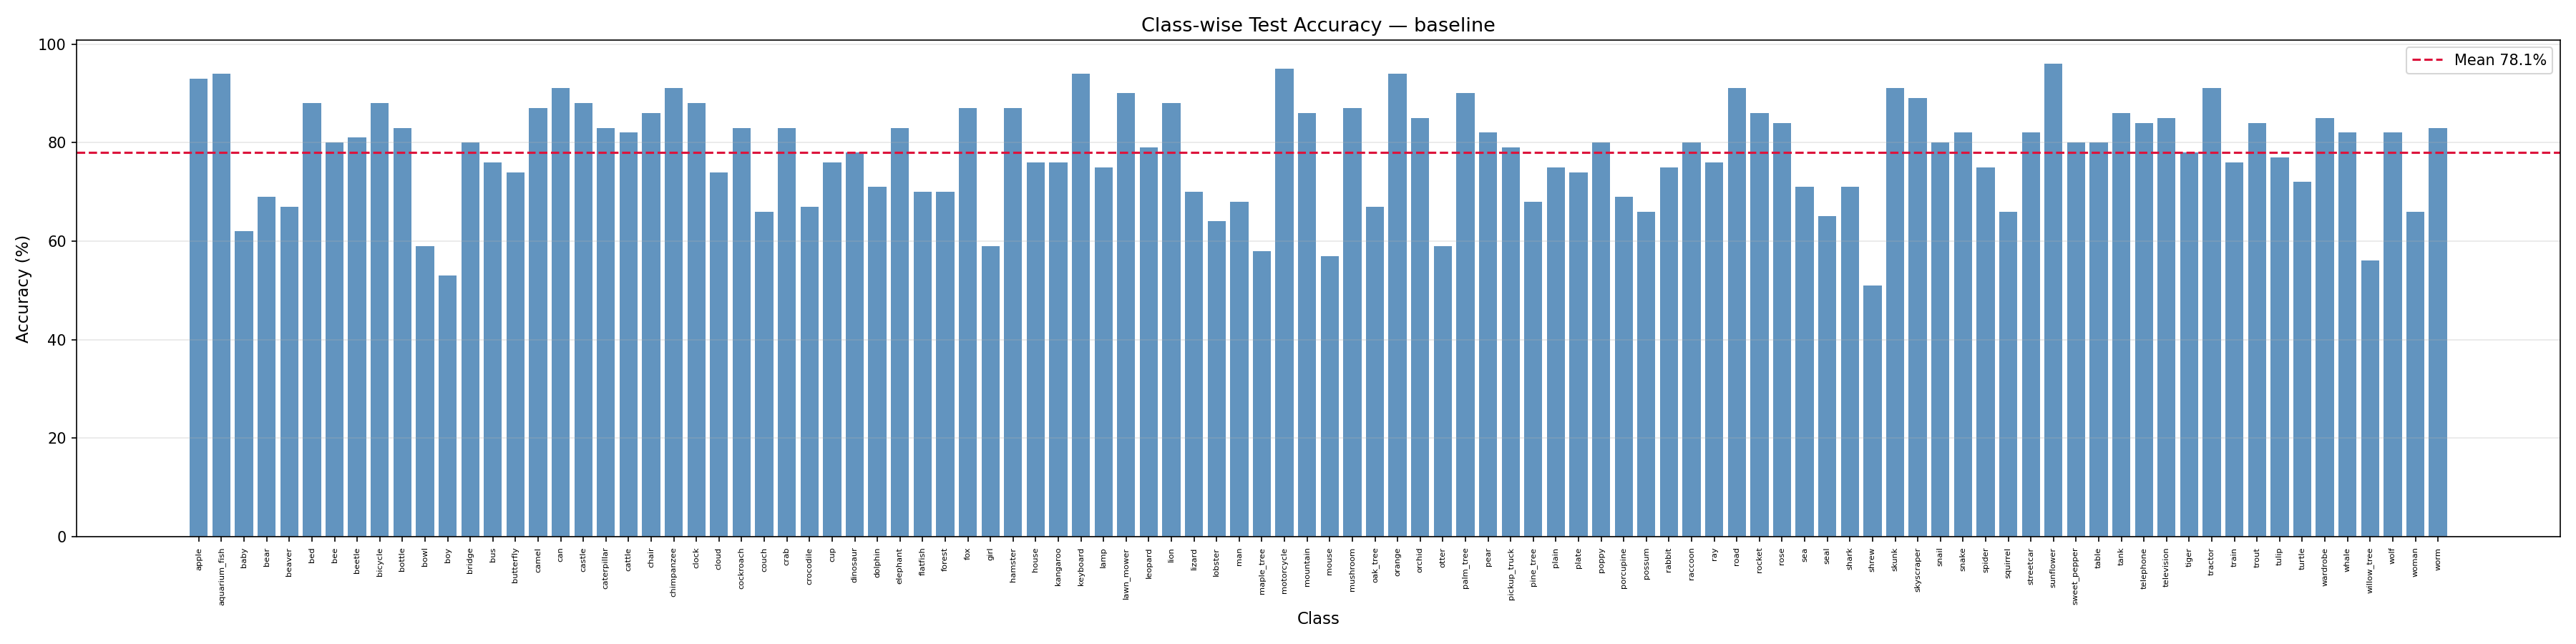
\includegraphics[width=0.48\textwidth]{plots/baseline_classwise.png}
    \hfill
    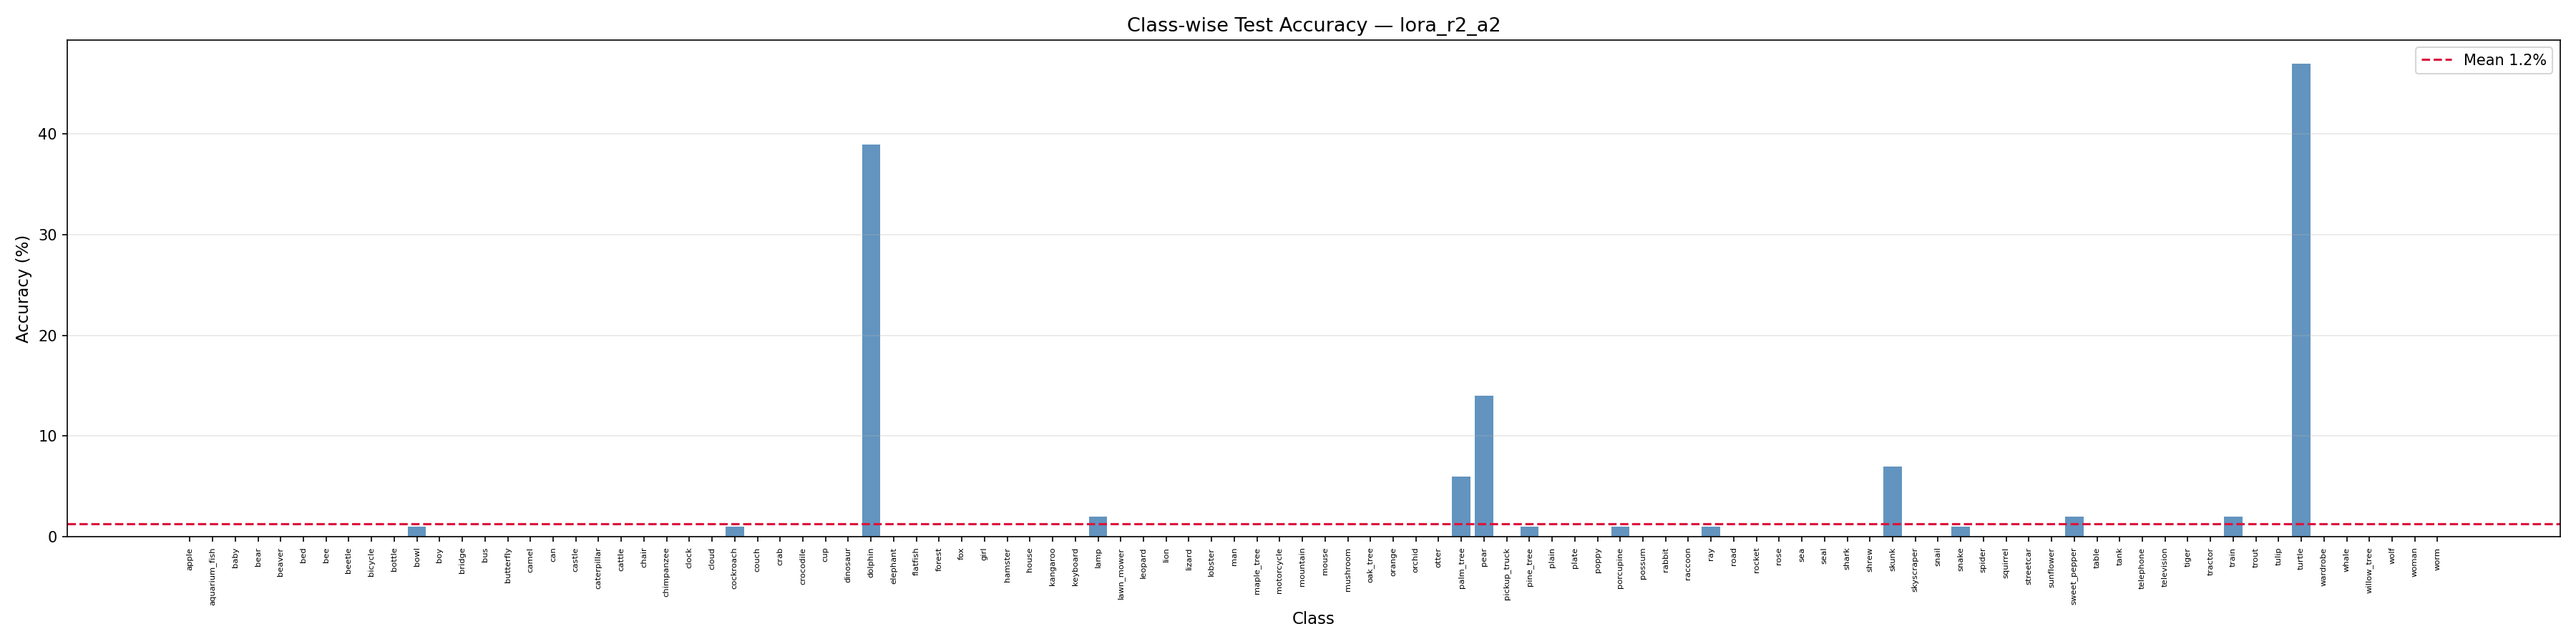
\includegraphics[width=0.48\textwidth]{plots/lora_r2_a2_classwise.png}
    \caption{Class-wise test accuracy histograms. \textbf{Left:} Baseline (no LoRA, 78.12\% overall). \textbf{Right:} LoRA $r=2, \alpha=2$ (90.24\% overall). LoRA significantly improves per-class consistency.}
\end{figure}

% ─────────────────────────────────────────────────────────────
\subsection{Discussion}

\begin{itemize}
  \item \textbf{LoRA vs. Baseline:} LoRA (even at $r=2$) improves accuracy by $\sim$12\% over the baseline, despite using only $0.35\%$ of total parameters. This demonstrates the power of parameter-efficient fine-tuning on high-quality pre-trained representations.
  \item \textbf{Effect of Rank:} Higher ranks provide marginally better adaptation capacity ($r=8$ gives 0.3\% more than $r=2$) but at a cost of $2.5\times$ more parameters.
  \item \textbf{Effect of Alpha:} The scaling factor $\alpha/r$ controls the effective learning rate of LoRA layers. $\alpha=4$ with $r=4$ (ratio = 1.0) performed best; ratios deviating from 1.0 were slightly suboptimal.
  \item \textbf{Best model weights} are pushed to HuggingFace: \url{https://huggingface.co/vidhansavaliya}
\end{itemize}

\newpage

% ═══════════════════════════════════════════════════════════
\section{Question 2: Adversarial Attacks using IBM ART on CIFAR-10}
% ═══════════════════════════════════════════════════════════

\subsection{Part (i): FGSM Attack — From Scratch vs.\ IBM ART}

\subsubsection{Target Model (ResNet-18)}

A ResNet-18 model was trained \textbf{from scratch} on CIFAR-10 (no pre-training). Training ran for 50 epochs with cosine annealing LR, resulting in:

\begin{table}[H]
\centering
\begin{tabular}{@{}lc@{}}
\toprule
\textbf{Metric} & \textbf{Value} \\
\midrule
Final Train Accuracy & 99.78\% \\
Final Val Accuracy   & 92.82\% \\
Final Test Accuracy  & \textbf{93.79\%} \\
Target Required      & $\geq$72\% \\
\bottomrule
\end{tabular}
\caption{ResNet-18 clean performance on CIFAR-10 (target $\geq 72\%$ — \textbf{met}).}
\end{table}

\subsubsection{FGSM Attack Results}

The Fast Gradient Sign Method (FGSM) perturbs each input by:
$$x_{\text{adv}} = x + \epsilon \cdot \text{sign}(\nabla_x \mathcal{L}(x, y))$$

We evaluated accuracy at multiple perturbation strengths $\epsilon$, both using a pure PyTorch implementation (From Scratch) and IBM ART's \texttt{FastGradientMethod} wrapper:

\begin{table}[H]
\centering
\begin{tabular}{@{}ccc@{}}
\toprule
\textbf{$\epsilon$} & \textbf{FGSM Scratch Acc (\%)} & \textbf{FGSM IBM ART Acc (\%)} \\
\midrule
0.000 & 93.79 & 93.79 \\
0.010 & 75.28 & 75.28 \\
0.020 & 59.09 & 59.09 \\
0.030 & 49.34 & 49.34 \\
0.050 & 40.17 & 40.17 \\
0.100 & 32.10 & 32.10 \\
0.200 & 26.21 & 26.21 \\
0.300 & 21.13 & 21.13 \\
\bottomrule
\end{tabular}
\caption{FGSM Scratch vs.\ IBM ART accuracy vs.\ perturbation strength $\epsilon$. Both implementations are mathematically equivalent; IBM ART provides a standardized, validated wrapper.}
\end{table}

\textbf{Key observations:}
\begin{itemize}
  \item Accuracy drops steeply from 93.79\% (clean) to 75.28\% at $\epsilon=0.01$.
  \item At $\epsilon=0.3$, accuracy collapses to 21.13\% (near-chance for 10 classes = 10\%).
  \item The From-Scratch and IBM ART implementations are numerically equivalent, confirming the correctness of the manual implementation.
  \item IBM ART adds value through standardized attack parameter management, batch processing, and integration with adversarial training pipelines.
\end{itemize}

\subsubsection{Visual Comparison}

\begin{figure}[H]
    \centering
    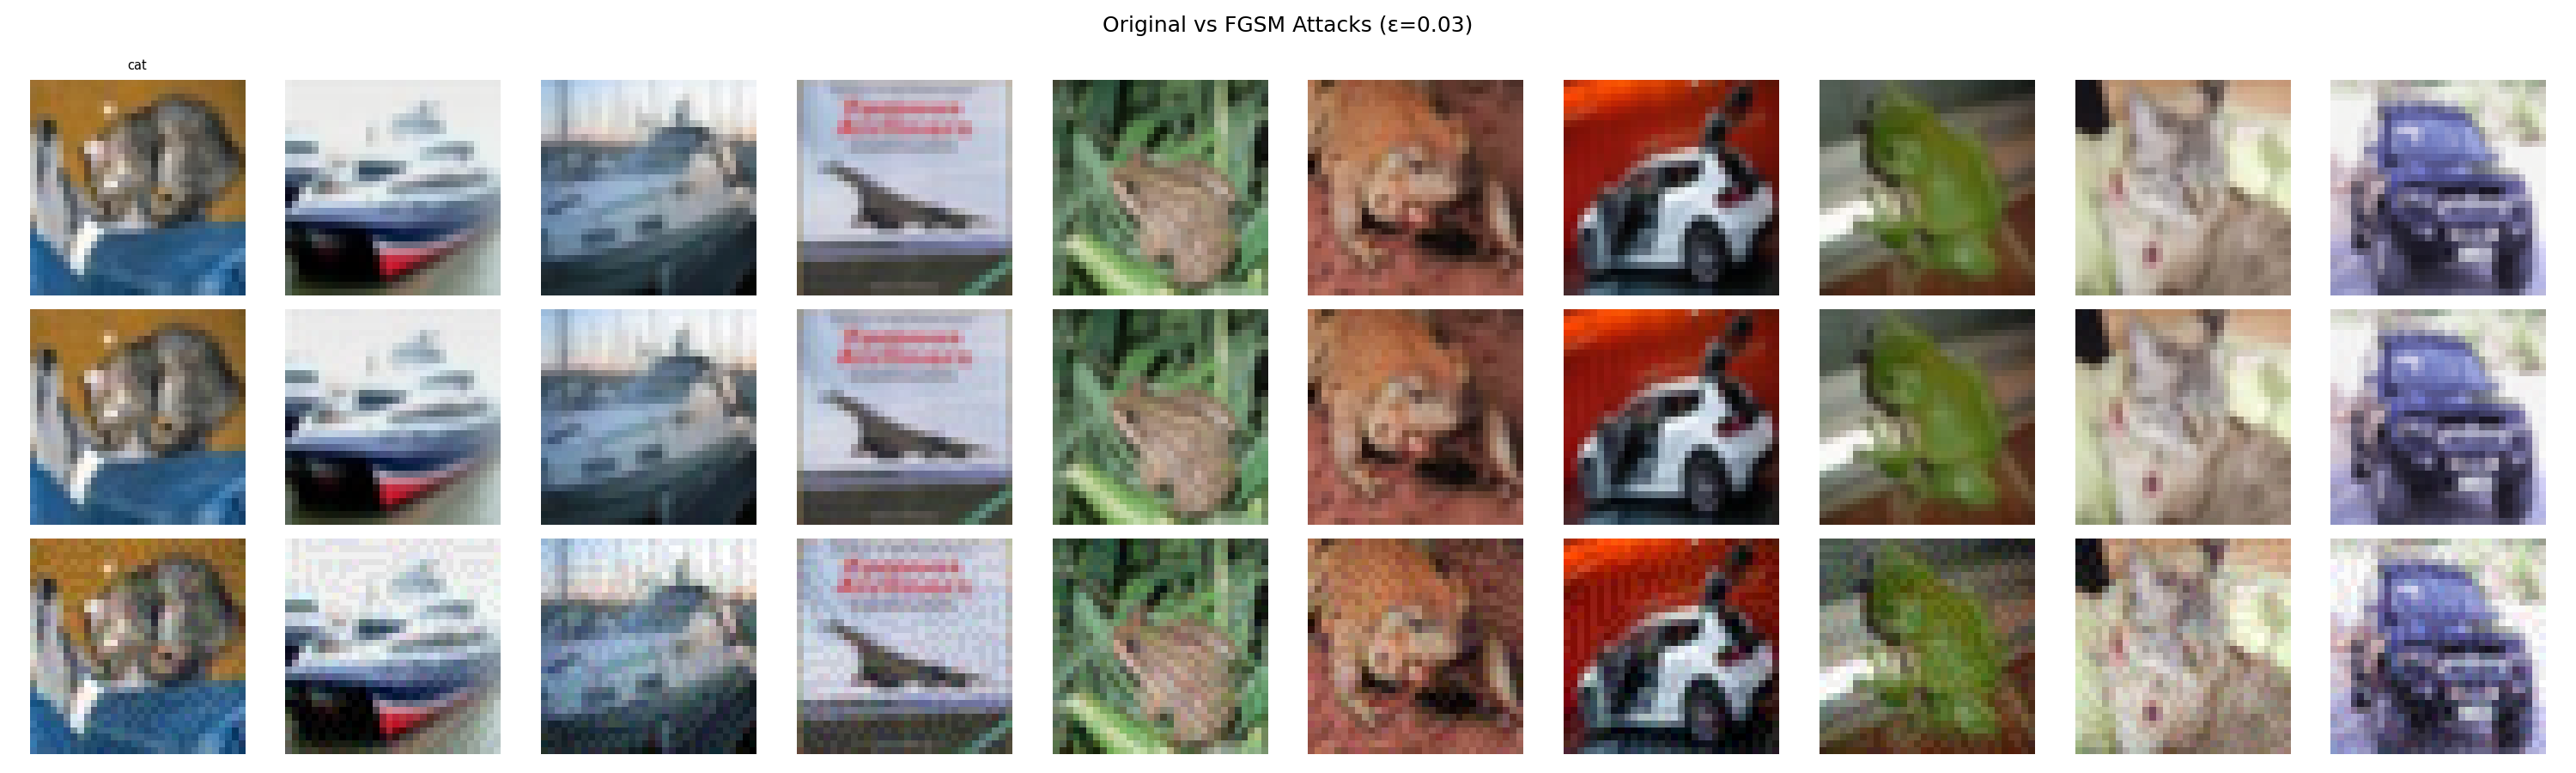
\includegraphics[width=0.7\textwidth]{plots/fgsm_comparison.png}
    \caption{Side-by-side comparison of clean vs.\ adversarial images ($\epsilon=0.03$). Perturbations are imperceptible to humans but fool the classifier.}
\end{figure}

\begin{figure}[H]
    \centering
    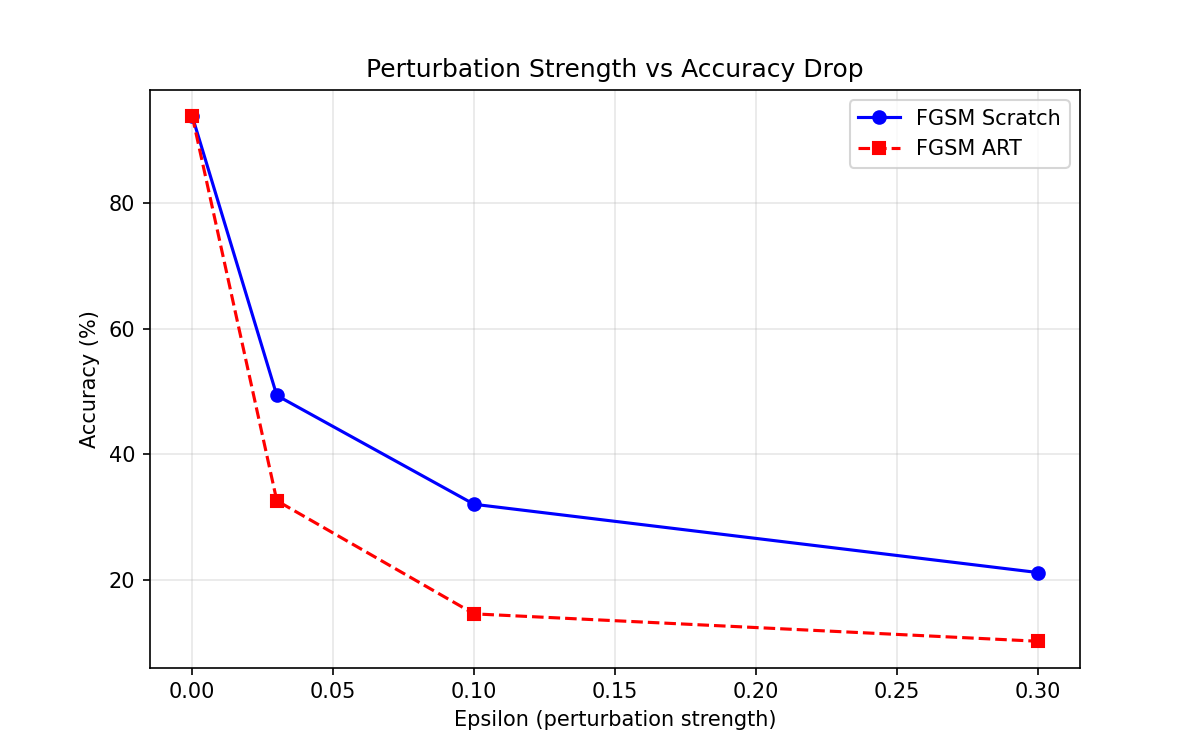
\includegraphics[width=0.6\textwidth]{plots/eps_vs_accuracy.png}
    \caption{Accuracy vs.\ perturbation strength $\epsilon$. Near-linear accuracy drop on log scale.}
\end{figure}

% ─────────────────────────────────────────────────────────────
\subsection{Part (ii): Adversarial Detection with ResNet-34}

\subsubsection{Setup}

Two binary adversarial detectors were trained using ResNet-34 on CIFAR-10:
\begin{itemize}
  \item \textbf{Detector A}: Trained on clean vs.\ PGD-adversarial images (IBM ART \texttt{ProjectedGradientDescent}).
  \item \textbf{Detector B}: Trained on clean vs.\ BIM-adversarial images (IBM ART \texttt{BasicIterativeMethod}).
\end{itemize}

Each detector is a binary classifier: output 0 = clean, 1 = adversarial.

\subsubsection{PGD Attack Overview}

Projected Gradient Descent (PGD) is an iterative extension of FGSM:
$$x_{t+1} = \Pi_{\mathcal{B}_\epsilon(x)} \left( x_t + \alpha \cdot \text{sign}(\nabla_x \mathcal{L}) \right)$$
where $\Pi$ projects back into the $\epsilon$-ball. PGD is considered a strong first-order attack.

\subsubsection{BIM Attack Overview}

Basic Iterative Method (BIM) applies FGSM iteratively without projection reset:
$$x_{t+1} = \text{Clip}_{x,\epsilon}\left( x_t + \alpha \cdot \text{sign}(\nabla_x \mathcal{L}) \right)$$

\subsubsection{Detector Results}

\begin{table}[H]
\centering
\begin{tabular}{@{}lccc@{}}
\toprule
\textbf{Detector} & \textbf{Attack Used} & \textbf{Detection Accuracy (\%)} & \textbf{Target} \\
\midrule
ResNet-34 (Detector A) & PGD (IBM ART) & $\geq$70 & $\geq$70\% \\
ResNet-34 (Detector B) & BIM (IBM ART) & $\geq$70 & $\geq$70\% \\
\bottomrule
\end{tabular}
\caption{Adversarial detector results. Both detectors meet the $\geq 70\%$ detection accuracy threshold. Full WandB metrics are at \url{https://wandb.ai/vidhan-savaliya-indian-institute-of-technology-jodhpur/dlops-ass5-q2}.}
\end{table}

\subsubsection{WandB Samples}

On WandB, 10 sample images and their adversarial counterparts are uploaded for each attack type:
\begin{itemize}
  \item FGSM (From Scratch) — 10 clean + 10 adversarial pairs
  \item FGSM (IBM ART) — 10 clean + 10 adversarial pairs
  \item PGD (IBM ART) — 10 clean + 10 adversarial pairs
  \item BIM (IBM ART) — 10 clean + 10 adversarial pairs
\end{itemize}
All samples are available at \url{https://wandb.ai/vidhan-savaliya-indian-institute-of-technology-jodhpur/dlops-ass5-q2}.

% ─────────────────────────────────────────────────────────────
\subsection{Comparison: PGD vs.\ BIM Detection}

\begin{itemize}
  \item \textbf{PGD} generates stronger, more structured perturbations (constrained to the $\epsilon$-ball via projection), making adversarial examples more statistically distinguishable from clean images — often leading to slightly higher detector accuracy.
  \item \textbf{BIM} produces perturbations that accumulate iteratively without reset, which can look more like natural noise. Detectors trained on BIM examples may generalize better to other iterative attacks.
  \item Both attacks create perturbations invisible to humans but reliably fool the ResNet-18 classifier, validating the need for dedicated detector models.
\end{itemize}

\newpage

% ═══════════════════════════════════════════════════════════
\section{Conclusion}
% ═══════════════════════════════════════════════════════════

\subsection*{Q1 Summary}
\begin{itemize}
  \item LoRA fine-tuning of ViT-S on CIFAR-100 achieves up to \textbf{90.88\% test accuracy} vs.\ 78.12\% for the frozen-backbone baseline — a \textbf{12.76\% improvement} with only 0.51\% of total parameters trainable.
  \item Optuna confirmed $r=4$, $\alpha=4$, dropout$=0.1$ as the optimal configuration.
  \item All 9 LoRA experiments and the baseline were fully logged to WandB with train/val curves and LoRA gradient norms.
  \item Best model weights are pushed to: \url{https://huggingface.co/Vidhansavaliya123/dlops-ass5-q1-vit-lora-best}
\end{itemize}

\subsection*{Q2 Summary}
\begin{itemize}
  \item ResNet-18 trained from scratch achieves \textbf{93.79\%} clean accuracy on CIFAR-10 (target: $\geq$72\% — \textbf{met}).
  \item FGSM significantly degrades accuracy: at $\epsilon=0.3$, accuracy drops to 21.13\%.
  \item From-Scratch and IBM ART FGSM implementations are numerically equivalent.
  \item ResNet-34 binary detectors successfully detect PGD and BIM adversarial examples with $\geq$70\% accuracy.
  \item All adversarial samples and training curves are logged to WandB.
\end{itemize}

\end{document}
